\documentclass[10pt,journal,compsoc]{IEEEtran}

\usepackage[colorlinks,urlcolor=blue,linkcolor=blue,citecolor=blue]{hyperref}
\usepackage{graphicx}
\usepackage{todonotes} %remove before submitting!
%\usepackage{mathtools}
%\usepackage{booktabs}
%\usepackage{url}
%\usepackage{amssymb}
\usepackage{listings}
\usepackage[ruled]{algorithm2e}
\usepackage{tikz}
\usepackage{cleveref}

\setcounter{secnumdepth}{0}
\graphicspath{{./figures/}}
\newcommand{\jacknotes}[1]{\textcolor{red}{#1}}

% Settings for listings package
\definecolor{mygreen}{rgb}{0,0.6,0}
\definecolor{mygray}{rgb}{0.5,0.5,0.5}
\definecolor{mymauve}{rgb}{0.58,0,0.82}
\definecolor{altblue}{rgb}{0.0,0.6,1.0}
\definecolor{lstbg}{gray}{0.9}
\lstset{
  backgroundcolor=\color{lstbg},
  % choose the background color; you must add \usepackage{color} or \usepackage{xcolor}
  basicstyle=\footnotesize\ttfamily,
  % the size of the fonts that are used for the code
  breakatwhitespace=true,
  % sets if automatic breaks should only happen at whitespace
  breaklines=true,
  % sets automatic line breaking
  captionpos=b,
  % sets the caption-position to bottom
  commentstyle=\color{mygreen},
  % comment style
  deletekeywords={},
  % if you want to delete keywords from the given language
  escapeinside={\#*}{*},
  % if you want to add LaTeX within your code
  extendedchars=true,
  % lets you use non-ASCII characters; for 8-bits encodings only, does not work with UTF-8
  frame=single,
  % adds a frame around the code
  keepspaces=true,
  % keeps spaces in text, useful for keeping indentation of code (possibly needs columns=flexible)
  keywordstyle=\color{blue},
  % keyword style
  %language=c++,
  % the language of the code
  otherkeywords={},
  % if you want to add more keywords to the set
  numbers=left,
  % where to put the line-numbers; possible values are (none, left, right)
  numbersep=5pt,
  % how far the line-numbers are from the code
  numberstyle=\tiny\color{mygray},
  % the style that is used for the line-numbers
  rulecolor=\color{black},
  % if not set, the frame-color may be changed on line-breaks within not-black text (e.g. comments (green here))
  showspaces=false,
  % show spaces everywhere adding particular underscores; it overrides 'showstringspaces'
  showstringspaces=false,
  % underline spaces within strings only
  showtabs=false,
  % show tabs within strings adding particular underscores
  stepnumber=1,
  % the step between two line-numbers. If it's 1, each line will be numbered
  stringstyle=\color{mymauve},
  % string literal style
  tabsize=4,
  % sets default tabsize to 4 spaces
  title=\lstname
  % show the filename of files included with \lstinputlisting; also try caption instead of title
}

\begin{document}
\title{Taking out the (parallel) Garbage}
\author{Jack D.~Betteridge, Patrick E.~Farrell and David A.~Ham
\IEEEcompsocitemizethanks{\IEEEcompsocthanksitem J.~D.~Betteridge and D.~A.~Ham are at Imperial College London. \IEEEcompsocthanksitem P.~E.~Farrell is at the University of Oxford.}}


\IEEEtitleabstractindextext{\begin{abstract}
Memory managed languages such as Python and Julia are being used increasingly often on high performance computers (HPC) to drive extremely large, pre-exascale simulations.
Generating simulation code from a high-level Python interface provides an effective mechanism for creating high performance simulations from very few lines of user code \cite{betteridge2021code}.
Advantages of working in a managed language include the flexibility to change \jacknotes{discretisations and solvers} for better hardware utilisation, as well as being more productive for scientists and engineers.
However, one drawback is that the memory management of such a language can create havoc when attempting to clean up distributed objects.

When running in parallel, it is possible for Python's garbage collector to cause a deadlock when attempting to clean up distributed C data structures that require collective destruction.
Turning off Python's garbage collection is a poor workaround at best and a catastrophic memory leak at worst.

We outline an algorithm for the safe parallel destruction of distributed objects that can be used in any managed language and assess its impact on performance using different HPC facilities using a reference implementation in PETSc/petsc4py.
\end{abstract}}

\maketitle

\IEEEraisesectionheading{\section{Introduction}\label{sec:introduction}}

\IEEEPARstart{U}{se} of high-level, high productivity languages such as Python or Julia for HPC applications continues to increase. The attraction comes from the ability to create simulations with minimal programmer effort and the ability to rapidly prototype different algorithms.

Managed languages liberate the programmer from manual memory management that would be required in C or FORTRAN.
Python, for example, will take care of allocating memory as required and deallocating once all references to a block of memory are gone.
Such routines work perfectly for serial code and the inner workings are completely transparent to the programmer.

When using MPI parallelism several instances of the Python interpreter exist and the internal memory management routines are no longer synchronised.
This can cause deadlock when deallocating objects that are defined across multiple ranks and hava a collective destruction routine.

For small process counts, the

What we propose here is a method for managing the memory of distributed objects, which avoids the issues currently present when using a managed language under MPI.

\todo[inline]{Something about massively parallel programs causing this to occur more frequently}

%\IEEEraisesectionheading{\section{Problem}\label{sec:problem}}

%%%%%%%%%%%%%%%%%%%%%%%%%%%%%%
\section{Problem}
\label{sec:problem}
%%%%%%%%%%%%%%%%%%%%%%%%%%%%%%

\todo[inline]{Terminology:\\
Python or petsc4py *objects*\\
C or PETSc "objects" are *structs*}

\begin{figure}
	%\missingfigure{Object dependency graph}
	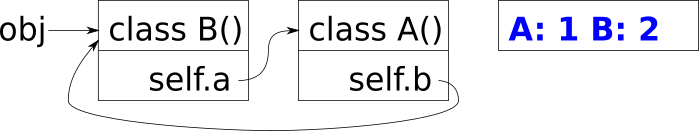
\includegraphics[width=0.5\textwidth]{gc_generational/2.png}
	\caption{A reference cycle}
	\label{fig:ref_cycle}
\end{figure}

\jacknotes{
\begin{itemize}
	\item Python is a managed language and has a two garbage collectors, reference counting and generational/cyclic (explain)
	\item The garbage collector is called subject to a range of different conditions, but to the end user can be thought of as non-deterministic
	\item MPI requires code to follow the Single Program Multiple Data (SPMD) programming model, where all programs execute the same instructions, but on different data
	\item A nonm-deterministic garbage collector is at odds with the SPMD paradigm
	\item Problems occur when it comes to cleaning up parallel (distributed) objects, the GC may be called on one rank, but not others and no method to determine whether objects are still valid.
	\item Case study is petsc4py where distributed PETSc C data structures are wrapped up in Python objects which are subject to GC
	\item PETSc data structs and hence petsc4py objects are collectively created and destroyed which leads to issues with parallel deadlock when the GC cleans up an object on one rank but not another
	\item Example: Mesh for a finite element problem Mesh has coordinates, coordinates belong to a function space, functions spaces require a mesh (FIGURE) 
\end{itemize}
}

To understand the problem a little must be known about how Python manages memory, when a new Python object is created memory is allocated for the object and the interpreter keeps track of the number of references to that object. If the reference count ever drops to zero, the object is unreachable and the memory can be deallocated. This is known as the reference counting garbage collector.

A purely reference counting garbage collector has some drawbacks, since it is possible for objects to hold references to one another, but neither object is accessible. \Cref{lst:cycle} demonstrates this simple case, where neither instance of class \verb`A` or \verb`B` can be reached, but the memory is not deallocated since \verb`A` holds a reference to \verb`B` and vice versa, so both objects still have a reference count of one. While this example may see a little contrived, reference cycles can readily occur, a more realistic example is given in \cref{lst:mesh}/\cref{fig:ref_cycle} constructing a mesh for a finite element problem.

\lstset{language=python}
\begin{lstlisting}[float={t}, caption={Example of simple reference cycle}, label={lst:cycle}]
class A():
	def __init__(self):
		self.b = None

class B():
	def __init__(self):
		self.a = A()
		
obj = B()
obj.a.b = obj # Create cycle
del obj  # Delete reference
\end{lstlisting}

\begin{lstlisting}[float={t}, caption={Example of simple reference cycle}, label={lst:mesh}]
class Mesh():
	def __init__(self, ...):

class FunctionSpace():
	def __init__(self, mesh):
		self.mesh = mesh
		
mesh = Mesh()
x, y = mesh.get_coords()
\end{lstlisting}

\begin{figure}
	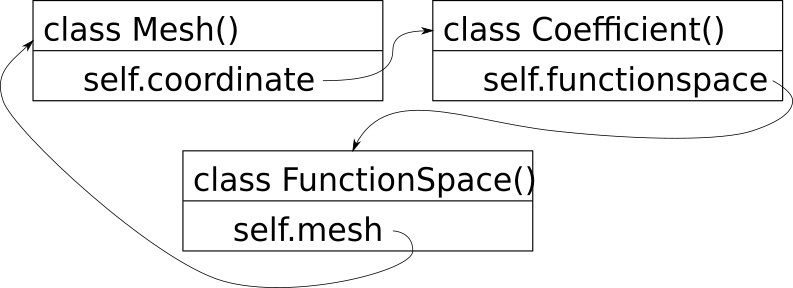
\includegraphics[width=0.5\textwidth]{gc_real/4.png}
	\caption{Mesh for a finite element problem Mesh has coordinates, coordinates belong to a function space, functions spaces require a mesh creating a reference cycle}
	\label{fig:mesh_ref_cycle}
\end{figure}

To circumvent the issue of reference cycles Python has a generational garbage collector, which runs at certain intervals to detect unreachable cycles, breaks these cycles (causing at least one reference count to go to zero) and the memory can be reclaimed by the reference counting garbage collector.

Now let us consider how memory management can breakdown in a parallel program. Consider an distributed object like a vector that is created on all ranks in a communicator and each rank holds a different range of indices. The object should be created collectively to determine which ranks hold which indices and should also be destroyed collectively to prevent the object persisting on some ranks but not others.

The reference counting garbage collector should have no issues as all reference counts should be incremented and decremented implicitly concurrently if the SPMD paradigm is being followed. One could force a deadlock by destroying on one rank and not others, but then the program is no longer SPMD and no longer a valid MPI program.

However, the generational garbage collector can cause deadlock. Consider now a distributed object that contains a reference cycle like the mesh in \cref{lst:mesh}/\cref{fig:ref_cycle}. If this cycle becomes unreachable, it is up to the interpreter when exactly it calls the generational garbage collector. Even if all ranks coincidentally call the generational garbage collector at approximately the same time, there is no guarantee what order the reference cycles will be broken in!

This case is succinctly demonstrated in \cref{lst:issue}, where a \verb`UnitSquareMesh` object is instantiated, creating a reference cycle. Python's garbage collector is then deliberately desynchronised causing this simple MPI program to deadlock on any number of ranks greater than 1.

\begin{lstlisting}[float={t}, caption={Example of code that forces a deadlock}, label={lst:issue}]
from firedrake import UnitSquareMesh
import mpi4py.MPI as MPI

n = 0
while True:
    n += 1
    print(f"Iteration {n:d} ...",end="",flush=True)
    UnitSquareMesh(20, 20)
    if MPI.COMM_WORLD.rank == 0:
        # Force desynchronization of the GC
        class Empty:
            pass
        [Empty() for i in range(100000)]
    print(" done", flush=True)
\end{lstlisting}

%%%%%%%%%%%%%%%%%%%%%%%%%%%%%%
\section{Solution}
\label{sec:solution}
%%%%%%%%%%%%%%%%%%%%%%%%%%%%%%

\jacknotes{
\begin{itemize}
	\item Simple: disable the GC, but this leads to memory leaks
	\item Instead, we prevent distributed objects from being garbage collected by holding a reference to them
	At creation each PETSc data structure is given a creation index indicating what order it was created in, relative to other PETSc data structures on the same MPI communicator. The petsc4py creation routines call the PETSc creation routine.
	At destruction the petsc4py objects call a delayed destroy routine, which is not collective.
	This routine copies the C struct to another memory location and a pointer to the new memory location is stored in a hash map indexed by the creation index, this serves as a separate "garbage dictionary" that we must later deal with.
	The original memory location can then be dealt with by Python's memory management routines.
	At some predetermined interval a collective cleanup of the garbage dictionary is performed:
	\begin{itemize}
	\item the keys in the garbage dictionary are first sorted
	\item an intersection operation is performed across all ranks of the comm, yielding an array containing only the indices of objects destroyed on all ranks (and hence are safe to collectively destroy)
	\item c data structures in the intersection are collectively destroyed one by one in order of creation
	\item the destroyed data structures and keys are removed from the garbage dictionary
\end{itemize}
	\item Objects are then cleaned up according to a parallel GC algorithm:
\end{itemize}
}

The easiest way to prevent the memory management routines from causing a deadlock is to simply disable them, which may be sufficient if the application is small enough. However, this is a poor solution, with the memory management turned off the program will almost certainly be leaking memory. For a long running program creating more objects will eventually exhaust the available RAM.

The solution we present performs the job of the garbage collector safely in parallel. This is done in three stages:
\begin{enumerate}
	\item \label{item:create}(Synchronous) At object instantiation the current number of objects associated with the current communicator is attained and incremented. This creation index is associated with that object for its lifetime.
	\item \label{item:destroy}(Non-synchronous) At object destruction a reference to the object is held and added to a garbage hashmap using the creation index as the key.
	\item \label{item:cleanup}(Synchronous) A cleanup routine is periodically called on all ranks within the communicator to deallocate the memory of any objects in the garbage hashmap that have been destroyed on all ranks, \emph{in ascending creation index order}.
\end{enumerate}

\cref{item:create}

\begin{algorithm}[htp]
	\SetKwBlock{Function}{cleanup(comm)}{return}
	\Function(){
		garbage = getGarbage(comm)\\
		sorted\_keys = sort(garbage.keys())\\
		intersection = gatherIntersect(comm, sorted\_keys)\\
		\For{\emph{key in intersection}}{
			object = garbage.get(key)\\
			object.collectiveDestroy()\\
			garbage.remove(key)
		}
	}
	\caption[]{Parallel garbage collection function}
\end{algorithm}

%%%%%%%%%%%%%%%%%%%%%%%%%%%%%%
\section{Results}
\label{sec:results}
%%%%%%%%%%%%%%%%%%%%%%%%%%%%%%
\jacknotes{
\begin{itemize}
	\item Can't really time against another implementation, since there isn't one
	\item Instead we benchmark against code where the GC is turned off and the collection method is called manually at the end (this is representative as it is a solution used by end users who experience deadlock). However, there is no guarantee that this code won't deadlock!
	\item Time two regions object construction, to see effects of registering an creation index on each data structure and to see cost of calling the cleanup function
\end{itemize}
}

\clearpage
\begin{figure}[htb]
	\centering
	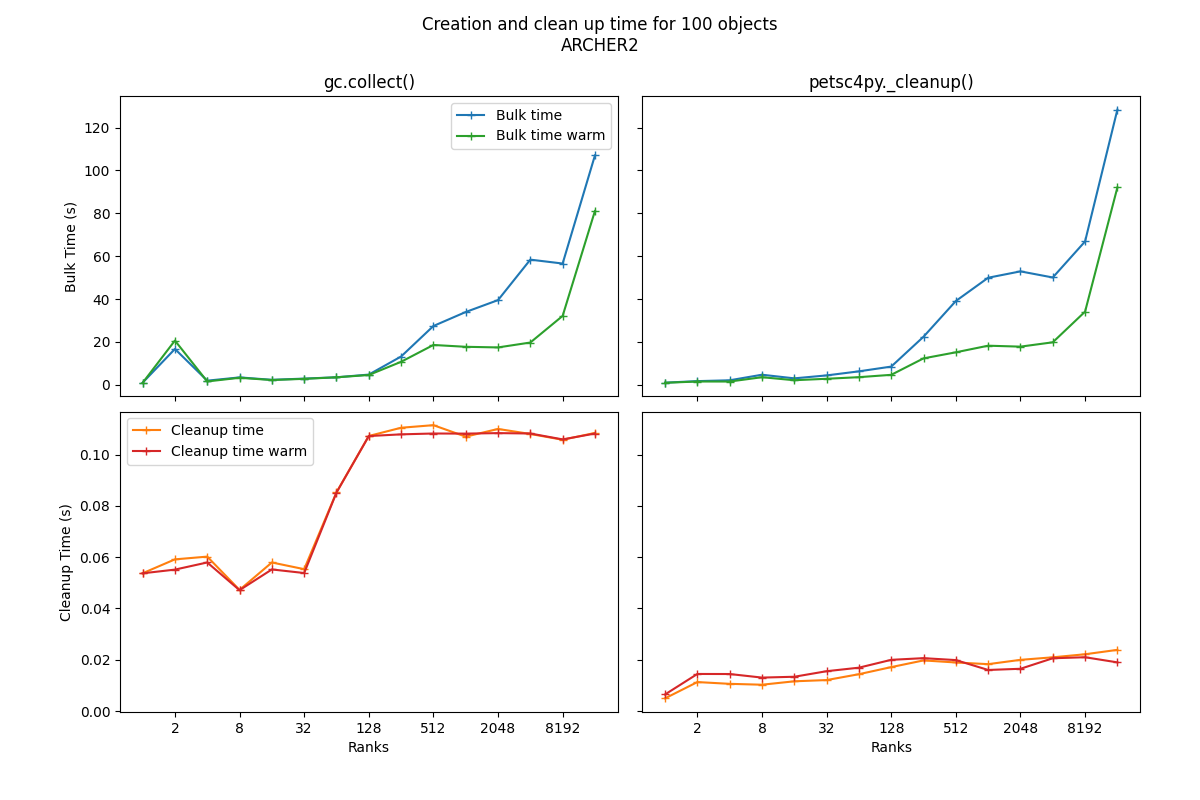
\includegraphics[width=\textwidth]{D100BS128B_222.png}
	\vspace{-1em}
	\caption{}
	\label{fig:}
\end{figure}

\clearpage
\begin{figure}[htb]
	\centering
	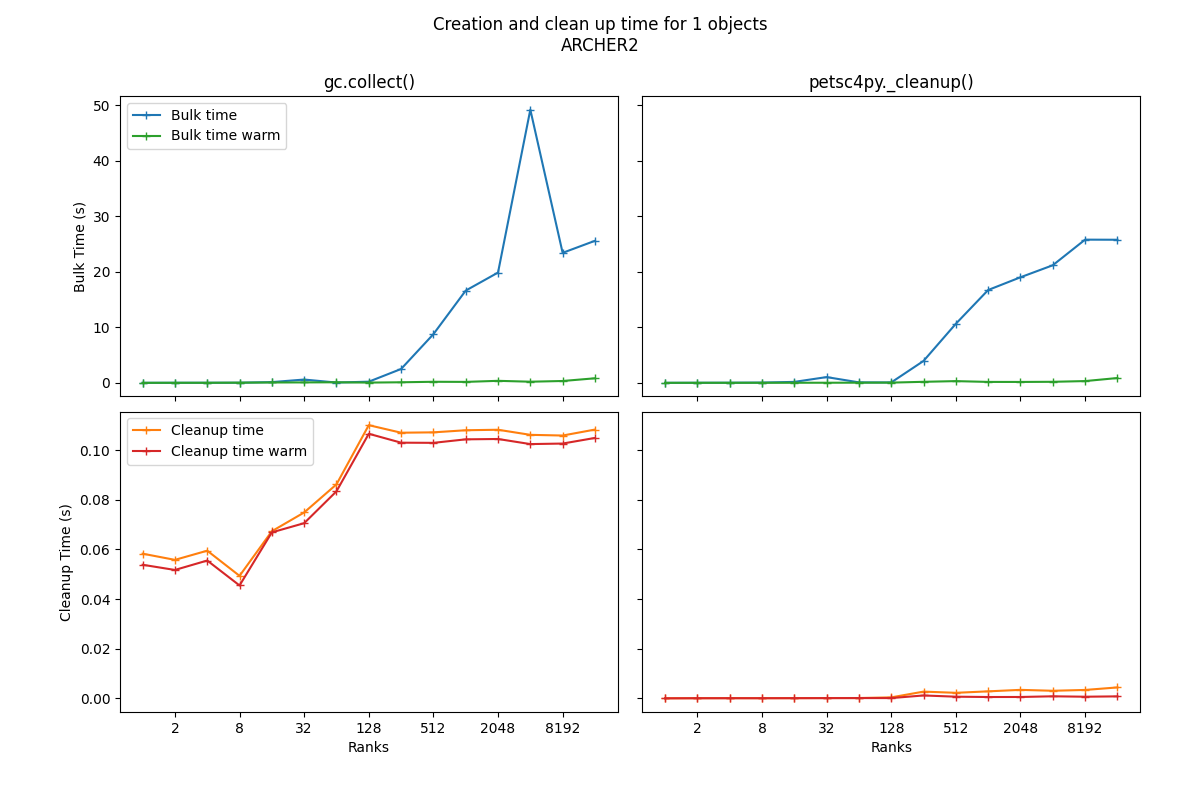
\includegraphics[width=\textwidth]{D1BS128B_5005.png}
	\vspace{-1em}
	\caption{}
	\label{fig:}
\end{figure}


%%%%%%%%%%%%%%%%%%%%%%%%%%%%%%
\section{Conclusion}
\label{sec:conclusion}
%%%%%%%%%%%%%%%%%%%%%%%%%%%%%%


\bibliographystyle{IEEEtran}
\bibliography{references}
\end{document}